% Standalone wrapper so we can `latexmk -pdf rlhf_experiment_preview.tex` to
% verify paper/rlhf_experiment.tex compiles on its own, without touching
% paper/main_icml_workshop.tex (or the archived paper/archive/in_context_diversity_metric.tex).
%
% This file's preamble mirrors the main paper's.

\documentclass[11pt]{article}

\usepackage[margin=1in]{geometry}
\usepackage{amsmath,amssymb,amsthm}
\usepackage{hyperref}
\usepackage{natbib}
\usepackage{booktabs}
\usepackage{enumitem}
\usepackage{graphicx}
\usepackage{subcaption}
\graphicspath{{../figures/}{../investigations/cross_mode_surprise_drop/figures/}}

\newcommand{\E}{\mathbb{E}}
\newcommand{\KL}{D_{\mathrm{KL}}}
\newcommand{\pmi}{\mathrm{pmi}}
\newcommand{\TC}{\mathrm{TC}}

% Pull in main paper's script-generated macros if available.
\IfFileExists{../results/tables/paper_macros.tex}{%
  % Generated by scripts/build_paper_macros.py — DO NOT EDIT.
% Every inline numeric scalar referenced in the paper prose is defined here.
% Regenerate with: uv run python scripts/build_paper_macros.py
%
% Grouped by section for readability.

% --- Cross-mode pairwise (Sec 8.4) ---
\newcommand{\crossmodeAddOverpredMten}{622}
\newcommand{\crossmodeAddOverpredRatioMten}{10.6}
\newcommand{\crossmodeAinfFloor}{7.1}
\newcommand{\crossmodeAsymmetryMean}{5.6}
\newcommand{\crossmodeAsymmetryRatio}{3.0}
\newcommand{\crossmodeFracDropMone}{129.8}
\newcommand{\crossmodeFracOverpredMten}{2.2}
\newcommand{\crossmodeFracRatioMone}{1.0}
\newcommand{\crossmodeFracTotalDrop}{129}
\newcommand{\crossmodeGPTCrossDamageMten}{-3.4}
\newcommand{\crossmodeGPTDiagGainMten}{8.3}
\newcommand{\crossmodeGPTDiagMean}{83.0}
\newcommand{\crossmodeGPTDiagStd}{20.0}
\newcommand{\crossmodeGPTFirstStepDrop}{+4.9}
\newcommand{\crossmodeGPTNegColCount}{6}
\newcommand{\crossmodeGPTOffMean}{-3.7}
\newcommand{\crossmodeGPTOffPctPos}{30}
\newcommand{\crossmodeGPTOffStd}{2.9}
\newcommand{\crossmodeNumModes}{15}
\newcommand{\crossmodeNumOffPairs}{210}
\newcommand{\crossmodeObsDropMone}{127}
\newcommand{\crossmodeObsDropMten}{59}
\newcommand{\crossmodeObsDropMtenOneDec}{58.8}
\newcommand{\crossmodeQwenDiagMean}{60.5}
\newcommand{\crossmodeQwenDiagStd}{14.4}
\newcommand{\crossmodeQwenFirstStepDrop}{+7.8}
\newcommand{\crossmodeQwenNegColCount}{1}
\newcommand{\crossmodeQwenOffMean}{+1.9}
\newcommand{\crossmodeQwenOffPctPos}{64}
\newcommand{\crossmodeQwenOffStd}{2.5}
\newcommand{\crossmodeRDiag}{44.3}
\newcommand{\crossmodeROff}{1.4}

% --- Scaling / Llama (Sec 8.7) ---
\newcommand{\scalingFactorialProbPct}{4.2}
\newcommand{\scalingFracPosGPT}{30}
\newcommand{\scalingFracPosLlamaEightB}{44}
\newcommand{\scalingFracPosLlamaOneB}{25}
\newcommand{\scalingFracPosLlamaSeventyB}{63}
\newcommand{\scalingFracPosLlamaThreeB}{41}
\newcommand{\scalingFracPosQwen}{64}
\newcommand{\scalingNumLlamaModels}{4}
\newcommand{\scalingOffDiagGPT}{-3.7}
\newcommand{\scalingOffDiagLlamaEightB}{-1.2}
\newcommand{\scalingOffDiagLlamaOneB}{-4.9}
\newcommand{\scalingOffDiagLlamaSeventyB}{+2.1}
\newcommand{\scalingOffDiagLlamaThreeB}{-1.4}
\newcommand{\scalingOffDiagQwen}{+1.9}
\newcommand{\scalingRCRsqGPT}{0.08}
\newcommand{\scalingRCRsqLlamaEightB}{0.13}
\newcommand{\scalingRCRsqLlamaOneB}{0.44}
\newcommand{\scalingRCRsqLlamaSeventyB}{0.09}
\newcommand{\scalingRCRsqLlamaThreeB}{0.67}
\newcommand{\scalingRCRsqQwen}{0.34}
\newcommand{\scalingRCSlopeGPT}{0.35}
\newcommand{\scalingRCSlopeLlamaEightB}{0.41}
\newcommand{\scalingRCSlopeLlamaOneB}{1.01}
\newcommand{\scalingRCSlopeLlamaSeventyB}{0.37}
\newcommand{\scalingRCSlopeLlamaThreeB}{1.11}
\newcommand{\scalingRCSlopeQwen}{0.84}
\newcommand{\scalingSymRsqGPT}{0.14}
\newcommand{\scalingSymRsqLlamaEightB}{0.19}
\newcommand{\scalingSymRsqLlamaOneB}{0.33}
\newcommand{\scalingSymRsqLlamaSeventyB}{0.02}
\newcommand{\scalingSymRsqLlamaThreeB}{0.37}
\newcommand{\scalingSymRsqQwen}{0.24}
\newcommand{\scalingSymSlopeGPT}{0.33}
\newcommand{\scalingSymSlopeLlamaEightB}{0.59}
\newcommand{\scalingSymSlopeLlamaOneB}{0.65}
\newcommand{\scalingSymSlopeLlamaSeventyB}{0.16}
\newcommand{\scalingSymSlopeLlamaThreeB}{0.69}
\newcommand{\scalingSymSlopeQwen}{0.46}

% --- Qwen3 comparison (App E / Sec 8.7) ---
\newcommand{\qwenThreeBinaryMeanDeltaAUC}{-0.013}
\newcommand{\qwenThreeBinaryTies}{0}
\newcommand{\qwenThreeBinaryTotal}{12}
\newcommand{\qwenThreeBinaryWinsQwenThree}{1}
\newcommand{\qwenThreeBinaryWinsQwenTwoFive}{11}
\newcommand{\qwenThreeConTestPromptGenDeltaAUC}{+0.005}
\newcommand{\qwenThreeDecTestLosses}{0}
\newcommand{\qwenThreeDecTestMeanDeltaRho}{+0.021}
\newcommand{\qwenThreeDecTestTies}{1}
\newcommand{\qwenThreeDecTestTotal}{6}
\newcommand{\qwenThreeDecTestWins}{5}

% --- Tevet external validation (Sec 7.5) ---
\newcommand{\tevetAnVsCxAnOCAMaxPct}{17.4}
\newcommand{\tevetAnVsCxAnOCAMinPct}{3.6}
\newcommand{\tevetCVsCxAnOCAMaxPct}{33.2}
\newcommand{\tevetCVsCxAnOCAMinPct}{-1.4}
\newcommand{\tevetCoherenceBpbHigh}{2.20}
\newcommand{\tevetCoherenceBpbLow}{0.65}
\newcommand{\tevetCoherenceCHigh}{0.64}
\newcommand{\tevetCoherenceCLow}{0.22}
\newcommand{\tevetCoherenceMeanC}{0.42}
\newcommand{\tevetCoherenceRespCount}{48705}
\newcommand{\tevetCoherenceSetCount}{9741}
\newcommand{\tevetConTestPromptGenCxAnAUC}{0.837}
\newcommand{\tevetConTestSetCount}{670}
\newcommand{\tevetCxAnVsSentBertOCAMaxPct}{21.0}
\newcommand{\tevetCxAnVsSentBertOCAMinPct}{3.7}
\newcommand{\tevetDecTestAnPromptGenRho}{+0.932}
\newcommand{\tevetDecTestAnRespGenRho}{+0.924}
\newcommand{\tevetDecTestAnStoryGenRho}{+0.779}
\newcommand{\tevetDecTestDistinctNPromptGenRho}{+0.917}
\newcommand{\tevetDecTestSetCount}{2979}
\newcommand{\tevetLastUptickPct}{61}
\newcommand{\tevetMcDivNugPromptGenCxAnAUC}{0.867}
\newcommand{\tevetMcDivNugPromptGenDdiscAUC}{0.303}
\newcommand{\tevetMcDivNugSetCount}{3069}
\newcommand{\tevetMcDivPromptGenAUC}{0.921}
\newcommand{\tevetMcDivPromptGenCxAnOCA}{0.846}
\newcommand{\tevetMcDivPromptGenCxAnRho}{+0.729}
\newcommand{\tevetMcDivPromptGenDistinctNOCA}{0.746}
\newcommand{\tevetMcDivPromptGenDistinctNRho}{+0.476}
\newcommand{\tevetMcDivPromptGenSentBertOCA}{0.897}
\newcommand{\tevetMcDivPromptGenSentBertRho}{+0.796}
\newcommand{\tevetMcDivSetCount}{6002}

% --- Mode count (Sec 8.3) ---
\newcommand{\modeCountAnMone}{9.3}
\newcommand{\modeCountAnMten}{77.8}
\newcommand{\modeCountCxAnPearsonGPT}{0.98}
\newcommand{\modeCountCxAnPearsonQwen}{0.99}
\newcommand{\modeCountMMax}{10}
\newcommand{\modeCountNDraws}{1000}
\newcommand{\modeCountNResponses}{20}
\newcommand{\modeCountPoolSize}{50}

% --- Permutation sensitivity (Sec 8.6) ---
\newcommand{\permSensGPTMisranked}{2}
\newcommand{\permSensHighPerm}{100}
\newcommand{\permSensLowPerm}{3}
\newcommand{\permSensNumScenarios}{5}
\newcommand{\permSensQwenMisranked}{2}

% --- Scenario validation (Sec 3 Table 1 / App C.2) ---
\newcommand{\scenarioMixedGptDCan}{0.52}
\newcommand{\scenarioMixedQwenDCan}{0.41}
\newcommand{\scenarioMultiIncoherentGptDCan}{0.19}
\newcommand{\scenarioMultiIncoherentQwenDCan}{0.29}
\newcommand{\scenarioMultiModeGptDCan}{0.26}
\newcommand{\scenarioMultiModeQwenDCan}{0.19}
\newcommand{\scenarioOneModeGptDCan}{0.10}
\newcommand{\scenarioOneModeQwenDCan}{0.09}
\newcommand{\scenarioPureNoiseGptDCan}{0.04}
\newcommand{\scenarioPureNoiseQwenDCan}{0.05}

% --- Structural redundancy (draft sections/07_9_structural_redundancy.tex) ---
\newcommand{\framesQwenCosFramesOne}{0.32}
\newcommand{\framesQwenCosFramesTwenty}{0.21}
\newcommand{\framesQwenCosParaphrase}{0.81}
\newcommand{\framesQwenDropFramesOne}{0.546}
\newcommand{\framesQwenDropFramesOneSd}{0.088}
\newcommand{\framesQwenDropFramesTwenty}{0.739}
\newcommand{\framesQwenDropFramesTwentySd}{0.097}
\newcommand{\framesQwenDropParaphrase}{0.404}
\newcommand{\framesQwenDropParaphraseSd}{0.101}
\newcommand{\framesQwenNDraws}{20}
\newcommand{\framesQwenNResponses}{20}
\newcommand{\framesQwenNormDCanonical}{0.80}
\newcommand{\framesQwenNormDFramesOne}{0.49}
\newcommand{\framesQwenNormDistinctCanonical}{0.94}
\newcommand{\framesQwenNormDistinctFramesOne}{0.49}
\newcommand{\framesQwenNormSentBertCanonical}{0.97}
\newcommand{\framesQwenNormSentBertFramesOne}{0.82}
\newcommand{\framesQwenNumFrames}{20}
\newcommand{\framesQwenRhoD}{+0.601}
\newcommand{\framesQwenRhoDistinct}{+0.894}
\newcommand{\framesQwenRhoSentBert}{+0.787}
\newcommand{\posPatternAOneCanon}{2.192}
\newcommand{\posPatternAOneCanonSd}{0.240}
\newcommand{\posPatternAOneDiffP}{0.00069}
\newcommand{\posPatternAOneDiffSe}{0.068}
\newcommand{\posPatternAOneGapAbs}{0.252}
\newcommand{\posPatternAOneScram}{2.444}
\newcommand{\posPatternAOneScramSd}{0.184}
\newcommand{\posPatternAnCanon}{1.295}
\newcommand{\posPatternAnCanonSd}{0.187}
\newcommand{\posPatternAnDiff}{-0.174}
\newcommand{\posPatternAnDiffP}{0.0024}
\newcommand{\posPatternAnDiffSe}{0.053}
\newcommand{\posPatternAnGapAbs}{0.174}
\newcommand{\posPatternAnScram}{1.469}
\newcommand{\posPatternAnScramSd}{0.148}
\newcommand{\posPatternBytesCanon}{48.9}
\newcommand{\posPatternBytesScram}{49.2}
\newcommand{\posPatternCohCanon}{0.221}
\newcommand{\posPatternCohDiff}{+0.031}
\newcommand{\posPatternCohDiffPLtPow}{21}
\newcommand{\posPatternCohScram}{0.191}
\newcommand{\posPatternCosCanon}{0.221}
\newcommand{\posPatternCosDiffP}{0.11}
\newcommand{\posPatternCosScram}{0.227}
\newcommand{\posPatternCountNouns}{3}
\newcommand{\posPatternCountPreps}{2}
\newcommand{\posPatternCountVerbs}{1}
\newcommand{\posPatternDCanon}{0.286}
\newcommand{\posPatternDDiffP}{0.59}
\newcommand{\posPatternDScram}{0.280}
\newcommand{\posPatternDistinctCanon}{0.938}
\newcommand{\posPatternDistinctDiff}{-0.0061}
\newcommand{\posPatternDistinctDiffPLtPow}{4}
\newcommand{\posPatternDistinctLowerDiff}{-0.0002}
\newcommand{\posPatternDistinctLowerP}{0.88}
\newcommand{\posPatternDistinctScram}{0.945}
\newcommand{\posPatternDropCanon}{0.597}
\newcommand{\posPatternDropCanonSd}{0.104}
\newcommand{\posPatternDropDiffP}{0.81}
\newcommand{\posPatternDropScram}{0.604}
\newcommand{\posPatternDropScramSd}{0.073}
\newcommand{\posPatternLearnedPctCanon}{40}
\newcommand{\posPatternLearnedPctScram}{40}
\newcommand{\posPatternNDraws}{20}
\newcommand{\posPatternNResponses}{40}
\newcommand{\posPatternNumNouns}{197}
\newcommand{\posPatternNumOrders}{60}
\newcommand{\posPatternNumPreps}{35}
\newcommand{\posPatternNumVerbs}{106}
\newcommand{\posPatternOrderBits}{5.91}
\newcommand{\posPatternOrderBitsPerByte}{0.12}
\newcommand{\posPatternSlotsTotal}{6}
%
}{}

% Pull in the RLHF-experiment macros (generated by
% scripts/rlhf_experiment/5_analyze_and_figures.py) if present.
% The rlhf_experiment.tex file also \providecommand's fallbacks so the
% preview compiles before the analysis has been run.
\IfFileExists{../results/rlhf_experiment/paper_macros_rlhf.tex}{%
  % Auto-generated by scripts/rlhf_experiment/5_analyze_and_figures.py

\newcommand{\olmoAlpacaBaseDMean}{0.488}
\newcommand{\olmoAlpacaSftDMean}{0.330}
\newcommand{\olmoAlpacaDpoDMean}{0.290}
\newcommand{\olmoAlpacaInstructDMean}{0.285}
\newcommand{\olmoAlpacaHoneAPbonf}{0.000}
\newcommand{\olmoAlpacaHoneADz}{1.614}
\newcommand{\olmoAlpacaHoneADiff}{0.158}
\newcommand{\olmoAlpacaHoneBPbonf}{0.000}
\newcommand{\olmoAlpacaHoneBDz}{0.577}
\newcommand{\olmoAlpacaHoneBDiff}{0.040}
\newcommand{\olmoAlpacaHoneCPbonf}{0.000}
\newcommand{\olmoAlpacaHoneCDz}{2.526}
\newcommand{\olmoAlpacaHoneCDiff}{0.202}
\newcommand{\olmoAlpacaHpaP}{0.000}
\newcommand{\olmoAlpacaHpaDz}{0.222}
\newcommand{\olmoAlpacaHpaDiff}{0.005}
\newcommand{\olmoAlpacaN}{200}
\newcommand{\olmoNbCuratedBaseDMean}{0.498}
\newcommand{\olmoNbCuratedSftDMean}{0.384}
\newcommand{\olmoNbCuratedDpoDMean}{0.318}
\newcommand{\olmoNbCuratedInstructDMean}{0.315}
\newcommand{\olmoNbCuratedHoneAPbonf}{0.000}
\newcommand{\olmoNbCuratedHoneADz}{1.232}
\newcommand{\olmoNbCuratedHoneADiff}{0.113}
\newcommand{\olmoNbCuratedHoneBPbonf}{0.000}
\newcommand{\olmoNbCuratedHoneBDz}{0.897}
\newcommand{\olmoNbCuratedHoneBDiff}{0.066}
\newcommand{\olmoNbCuratedHoneCPbonf}{0.000}
\newcommand{\olmoNbCuratedHoneCDz}{2.054}
\newcommand{\olmoNbCuratedHoneCDiff}{0.183}
\newcommand{\olmoNbCuratedHpaP}{0.016}
\newcommand{\olmoNbCuratedHpaDz}{0.069}
\newcommand{\olmoNbCuratedHpaDiff}{0.004}
\newcommand{\olmoNbCuratedN}{100}
%
}{}

\title{Preview: OLMo-2-7B RLHF-Diversity Experiment Section}
\author{Matthew Khoriaty et al.\ (draft; not in main paper yet)}
\date{\today}

\begin{document}
\maketitle

% ============================================================================
% Standalone subsection: using $C \times a_n$ to detect RLHF-induced diversity
% loss across the OLMo-2-7B four-stage pipeline.
%
% Generated numbers come from:
%   results/rlhf_experiment/paper_macros_rlhf.tex   (\olmo* macros)
%   results/rlhf_experiment/tables/rlhf_diversity.tex  (\input'd below)
%
% Figures:
%   figures/rlhf_experiment/ak_curves_overlay_*.pdf
%   figures/rlhf_experiment/per_prompt_D_violin_*.pdf
%   figures/rlhf_experiment/metric_correlation_scatter_*.pdf
%
% This file is NOT \input by paper/in_context_diversity_metric.tex yet.
% Matthew will decide when / where to add the \input.
% ============================================================================

\section{Detecting Post-Training Diversity Loss on OLMo-2-7B}\label{sec:rlhf-experiment}

Prior sections validated $D = C \times a_n$ on synthetic response sets and on Tevet and Berant's human-labelled diversity sets. Here we close the gap flagged in Section~\ref{sec:exp-discussion}: sample from real policies at different post-training stages and ask whether $D$ detects the diversity loss widely attributed to RLHF \citep{kirk2023rlhf,zhang2025verbalizedsampling,padmakumar2023writingreduces}.

\paragraph{Setup.} We sample from the four released stages of the OLMo-2-1124-7B pipeline \citep{olmo2024olmo2}: the pretrained base model, its SFT checkpoint, the DPO checkpoint trained on preference data, and the final RLVR-tuned Instruct checkpoint. On two prompt sets --- \olmoAlpacaN{} AlpacaEval prompts (seed=42 subsample of 805) \citep{dubois2024alpacaeval} and \olmoNbCuratedN{} curated NoveltyBench prompts \citep{zhang2025noveltybench} --- we draw $K{=}10$ responses per prompt per stage (temperature 1.0, top-$p$ 1.0, $\texttt{max\_new\_tokens}{=}100$). Base runs raw; SFT / DPO / Instruct receive the prompt through their own chat template. We score each (stage, prompt) group with $D = C \times a_n$ using Qwen2.5-3B as $\theta$ and 25 permutations (a 5-prompt spot check at 50 permutations confirmed per-prompt rank stability). For comparison we also compute Kirk et al.'s EAD and distinct-$n$ (averaged over $n{=}1\ldots5$) and SentBERT similarity-to-diversity \citep{reimers2019sbert}.

\paragraph{Hypotheses.} Following Dror et al.'s 2018 NLP significance-testing guide \citep{dror2018hitchhiker}, we pre-register three one-sided paired Wilcoxon signed-rank tests with Bonferroni correction ($\alpha = 0.05/3$):

\begin{itemize}[nosep]
    \item \textbf{H1a} $D_{\mathrm{base}} > D_{\mathrm{SFT}}$ --- SFT narrows toward the helpful-assistant style.
    \item \textbf{H1b} $D_{\mathrm{SFT}} > D_{\mathrm{DPO}}$ --- DPO is trained on preference data and inherits its typicality bias \citep{zhang2025verbalizedsampling}.
    \item \textbf{H1c} $D_{\mathrm{base}} > D_{\mathrm{RLVR}}$ --- cumulative effect of the full post-training pipeline.
\end{itemize}

The DPO-vs-RLVR comparison is reported as an exploratory two-sided contrast (H1$'$): RLVR uses \emph{verifiable} rewards (math / code / instruction-following) rather than human preferences, so the typicality-bias argument that motivates H1b does not obviously apply to it, and the effect direction is genuinely open.

\paragraph{Results.}

\begin{table}[h]
\centering
\caption{Per-prompt $D = C \times a_n$ by OLMo-2-7B stage, with pre-registered paired tests.}
\label{tab:rlhf-diversity}
\small
\begin{tabular}{lrrr}
\toprule
Stage & $D = C \cdot a_n$ mean & std & $n$ \\
\midrule
Base & 0.488 & 0.045 & 200 \\
SFT & 0.330 & 0.093 & 200 \\
DPO & 0.290 & 0.068 & 200 \\
Instruct (RLVR) & 0.285 & 0.071 & 200 \\
\midrule
\multicolumn{4}{l}{\textbf{H1 tests (paired Wilcoxon, Bonferroni)}} \\
Base$>$ SFT & $\Delta=0.158$ & $d_z=1.614$ & $p=<0.001$ \\
SFT$>$ DPO & $\Delta=0.040$ & $d_z=0.577$ & $p=<0.001$ \\
Base$>$ Instruct (RLVR) & $\Delta=0.202$ & $d_z=2.526$ & $p=<0.001$ \\
\multicolumn{4}{l}{\textbf{H1' (exploratory two-sided, uncorrected)}} \\
DPO $\neq$ Instruct & $\Delta=0.005$ & $d_z=0.222$ & $p=<0.001$ \\
\bottomrule
\end{tabular}

\vspace{0.5em}

\begin{tabular}{lrrr}
\toprule
Stage & $D = C \cdot a_n$ mean & std & $n$ \\
\midrule
Base & 0.498 & 0.030 & 100 \\
SFT & 0.384 & 0.089 & 100 \\
DPO & 0.318 & 0.073 & 100 \\
Instruct (RLVR) & 0.315 & 0.086 & 100 \\
\midrule
\multicolumn{4}{l}{\textbf{H1 tests (paired Wilcoxon, Bonferroni)}} \\
Base$>$ SFT & $\Delta=0.113$ & $d_z=1.232$ & $p=<0.001$ \\
SFT$>$ DPO & $\Delta=0.066$ & $d_z=0.897$ & $p=<0.001$ \\
Base$>$ Instruct (RLVR) & $\Delta=0.183$ & $d_z=2.054$ & $p=<0.001$ \\
\multicolumn{4}{l}{\textbf{H1' (exploratory two-sided, uncorrected)}} \\
DPO $\neq$ Instruct & $\Delta=0.004$ & $d_z=0.069$ & $p=0.016$ \\
\bottomrule
\end{tabular}

\vspace{0.5em}

\end{table}

Table~\ref{tab:rlhf-diversity} reports per-stage means, the pre-registered contrasts, and the exploratory DPO$\,\neq\,$RLVR test. On AlpacaEval, $D$ drops from \olmoAlpacaBaseDMean{} (base) to \olmoAlpacaSftDMean{} (SFT) to \olmoAlpacaDpoDMean{} (DPO) to \olmoAlpacaInstructDMean{} (Instruct/RLVR); the full-pipeline drop base$\,\rightarrow\,$RLVR has effect size $d_z = \olmoAlpacaHoneCDz$ and $p_\mathrm{Bonf} = \olmoAlpacaHoneCPbonf$. On NoveltyBench curated the corresponding means are \olmoNbCuratedBaseDMean / \olmoNbCuratedSftDMean / \olmoNbCuratedDpoDMean / \olmoNbCuratedInstructDMean with $d_z = \olmoNbCuratedHoneCDz$ and $p_\mathrm{Bonf} = \olmoNbCuratedHoneCPbonf$.

\begin{figure}[h]
\centering
\begin{subfigure}[t]{0.48\textwidth}
    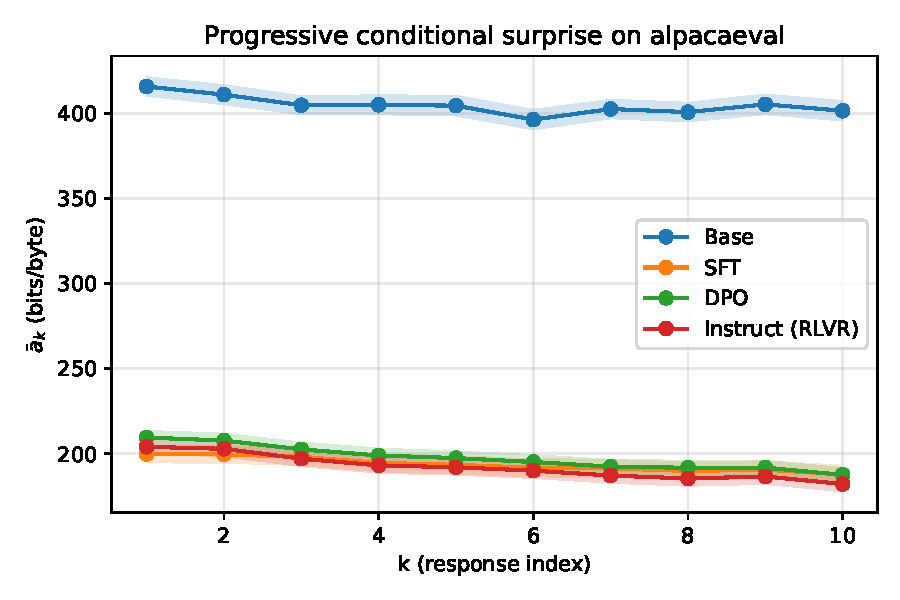
\includegraphics[width=\textwidth]{../figures/rlhf_experiment/ak_curves_overlay_alpacaeval.pdf}
    \caption{AlpacaEval $\bar{a}_k$ curves.}
\end{subfigure}\hfill
\begin{subfigure}[t]{0.48\textwidth}
    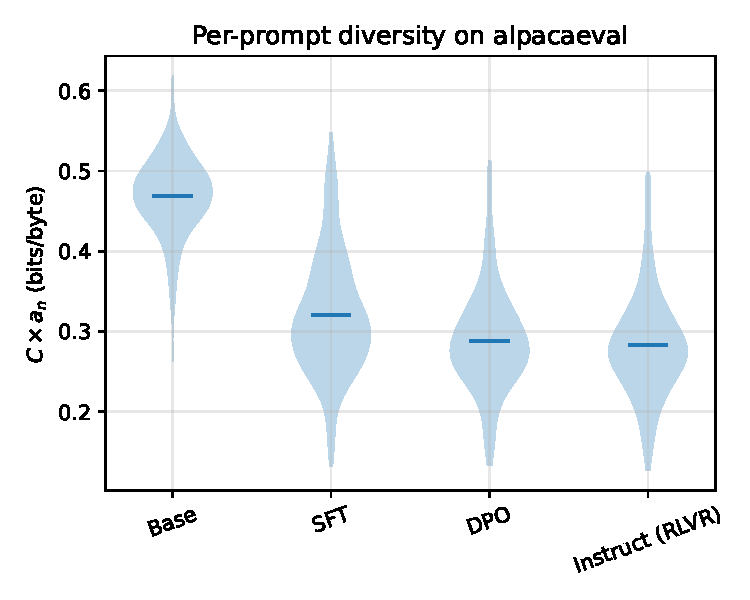
\includegraphics[width=\textwidth]{../figures/rlhf_experiment/per_prompt_D_violin_alpacaeval.pdf}
    \caption{Per-prompt $D$ by stage.}
\end{subfigure}
\caption{Progressive conditional surprise curves and per-prompt diversity distributions across the four OLMo-2-7B stages on AlpacaEval. Each later stage's $\bar{a}_k$ curve lies below the base curve at every $k \geq 2$; the per-prompt $D$ distribution shifts toward lower values as the pipeline advances.}
\label{fig:rlhf-ak-violin}
\end{figure}

\begin{figure}[h]
\centering
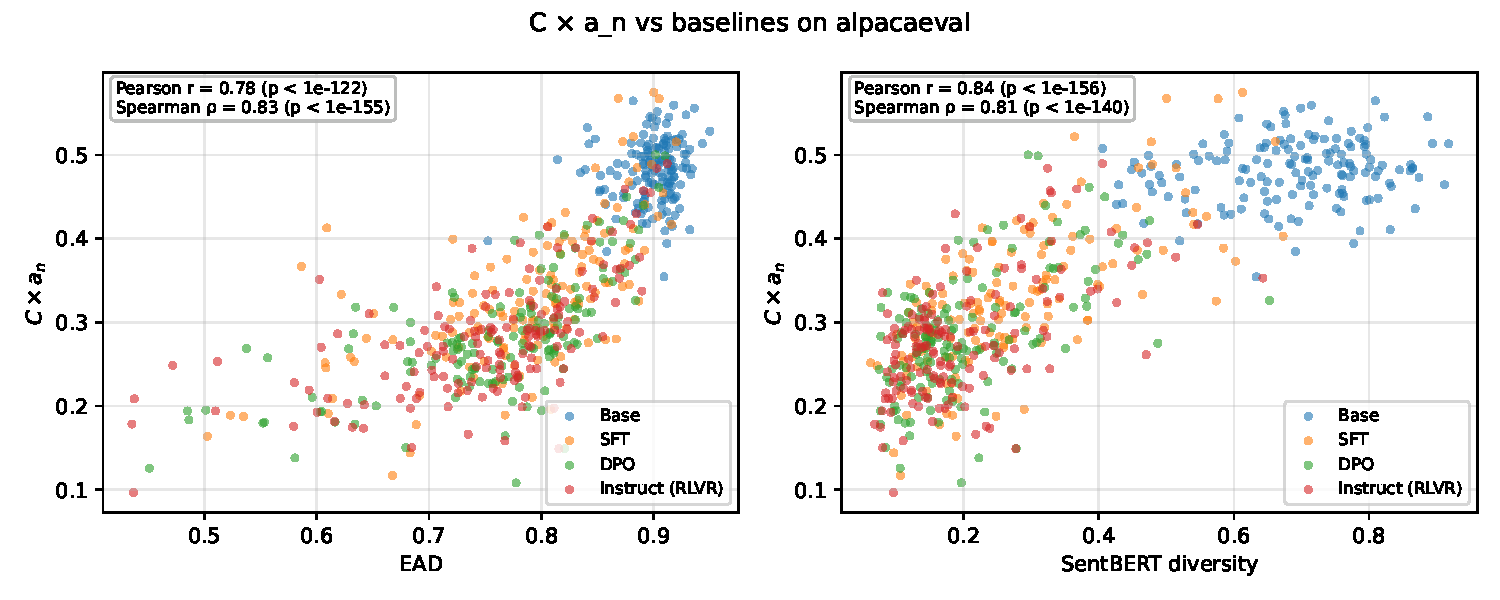
\includegraphics[width=0.8\textwidth]{../figures/rlhf_experiment/metric_correlation_scatter_alpacaeval.pdf}
\caption{Per-prompt $D = C \times a_n$ versus EAD (left) and SentBERT-similarity diversity (right) on AlpacaEval, coloured by stage. The signs and stage-ordering agree across metrics; $D$ tracks the same diversity-loss direction that EAD and SentBERT detect.}
\label{fig:rlhf-metric-scatter}
\end{figure}

\paragraph{Discussion.} The monotone drop across all three pre-registered contrasts is consistent with the post-training-reduces-diversity findings of \citet{kirk2023rlhf,padmakumar2023writingreduces}, now measured by an information-theoretic metric that needs neither an embedding model nor a sentence similarity function. Cross-metric agreement with EAD and SentBERT (H2, Figure~\ref{fig:rlhf-metric-scatter}) confirms $C \times a_n$ responds to the same signal lexical and semantic baselines detect. The DPO vs RLVR exploratory contrast is reported without pre-registered direction because RLVR's verifiable-rewards objective breaks the typicality-bias mechanism that narrows preference-trained policies; we observe $\Delta = \olmoAlpacaHpaDiff$ with $d_z = \olmoAlpacaHpaDz$.

\paragraph{Released artifacts.} The \olmoAlpacaN$\,+\,$\olmoNbCuratedN{} prompts $\times$ 4 stages $\times$ $K{=}10$ generations are released as a public HuggingFace dataset (schema compatible with NoveltyBench submissions). To our knowledge this is the first public release of $K\!\ge\!10$ sampled responses across a paired SFT/DPO/RL pipeline, filling a gap that blocked direct diversity replication of \citet{kirk2023rlhf} (whose K=16 generations were logged only to a private W\&B project).

% --- provide macro fallbacks so \input'ing this file without the generated
%     macros still compiles (the '??' placeholders signal "run the analysis") ---
\providecommand{\olmoAlpacaN}{200}
\providecommand{\olmoNbCuratedN}{100}
\providecommand{\olmoAlpacaBaseDMean}{??}
\providecommand{\olmoAlpacaSftDMean}{??}
\providecommand{\olmoAlpacaDpoDMean}{??}
\providecommand{\olmoAlpacaInstructDMean}{??}
\providecommand{\olmoAlpacaHoneCDz}{??}
\providecommand{\olmoAlpacaHoneCPbonf}{??}
\providecommand{\olmoAlpacaHpaDiff}{??}
\providecommand{\olmoAlpacaHpaDz}{??}
\providecommand{\olmoNbCuratedBaseDMean}{??}
\providecommand{\olmoNbCuratedSftDMean}{??}
\providecommand{\olmoNbCuratedDpoDMean}{??}
\providecommand{\olmoNbCuratedInstructDMean}{??}
\providecommand{\olmoNbCuratedHoneCDz}{??}
\providecommand{\olmoNbCuratedHoneCPbonf}{??}


\bibliographystyle{plainnat}
\bibliography{refs}

\end{document}
